\documentclass{beamer}
\usepackage{cmap}
\usepackage[utf8]{inputenc}
\usepackage[russian]{babel}
\usepackage{listings}
\usetheme{Antibes}
\usecolortheme{beaver}
\usepackage{graphicx}
\graphicspath{{img/}}

\title{Сегментация текста в проекте Открытый корпус}
\author{В.\,В.~Бочаров\andС.\,В.~Алексеева\andД.\,В.~Грановский\andН.\,А.~Остапук\andМ.\,Е.~Степанова\andА.\,В.~Суриков\\\small\it OpenCorpora.org}
\date{2~июня 2012~г.}
\begin{document}

% title page
\maketitle

%slide 01
\begin{frame}
\frametitle{О проекте Открытый Корпус}
\begin{enumerate}
\item{Цели}
    \begin{itemize}
    \item{для задач машинного обучения}
    \item{доступный под свободной лицензией}
    \item{с качественной ручной разметкой}
    \end{itemize}
\item{Ограничения}
    \begin{itemize}
    \item{маленький размер}
    \item{не сбалансирован}
    \end{itemize}
\item{На настоящий момент}
    \begin{itemize}
    \item{680K слов}
    \item{токенизирован вручную}
    \item{границы предложений проставлены вручную}
    \item{начата морфологическая разметка}
    \end{itemize}
\end{enumerate}
\end{frame}

%slide 03
\begin{frame}
\frametitle{Токенизация}
Как разделить текст на эти единицы?
\begin{itemize}
\item{на абзацы~-- взять из источника}
\item{на предложения~-- пока вручную}
\item{на токены~-- полуавтоматически}
\end{itemize}
\end{frame}

%slide 03.1
\begin{frame}
\frametitle{Токенизация}
Токенизация должна быть:
\begin{itemize}
\item{единообразной}
\item{удобной для морфологии}
\end{itemize}
Проблемы ручной токенизации:
\begin{itemize}
\item{очень трудоемко}
\item{трудно обеспечить единообразие}
\item{не все отличия видны глазами}
\end{itemize}
\end{frame}

%slide 04
\begin{frame}
\frametitle{Токенизация-2}
Используем простое машинное обучение:
\begin{itemize}
\item{корпус предложений, уже разделенных на токены (внутри текста расставлены границы)}
\item{набор бинарных характеристических функций (15 шт.)} \\
F1 = <<является ли данный символ пробелом>> \\
... \\
F7 = <<является ли данный символ буквой кириллицы>> \\
... \\
F15 = <<является ли цепочка символов от ближайшего пробела слева до ближайшего пробела справа словарным словом>>
\item{вычисляем все эти функции для каждой позиции в предложении}
\end{itemize}
\end{frame}

%slide 05
\begin{frame}
\frametitle{Токенизация-3}
Используем простое машинное обучение:
\begin{itemize}
\item{для каждой позиции получается двоичный вектор} \\
Позиция 1: 001000010000000 \\
Позиция 2: 100000100000010 \\
...
\item{для каждой позиции знаем, проходит ли в ней граница токенов}
\item{для каждого двоичного вектора на корпусе вычисляется вероятность того, что в позиции с таким вектором есть граница токенов}
\item{в реальном тексте в каждой позиции тоже вычисляем вектор и смотрим вероятность}
\end{itemize}
\end{frame}

%slide 06
\begin{frame}
\frametitle{Токенизация-4}
Так выглядит обучение:
\begin{figure}
\center{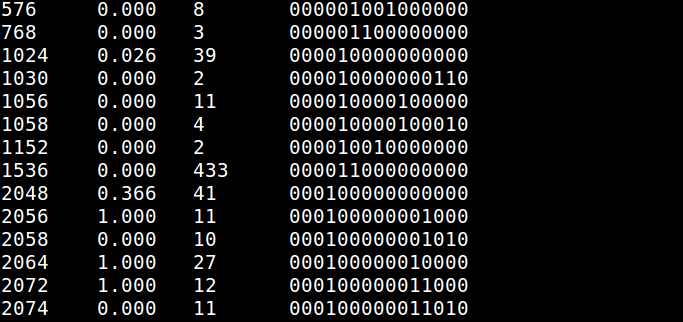
\includegraphics[width=1\linewidth]{2011_nlpseminar_1.png}}
\end{figure}
\end{frame}

%slide 07
\begin{frame}
\frametitle{Токенизация-5}
Получаемое деление~-- вероятностное, поэтому его нужно проверять глазами:
\begin{figure}
\center{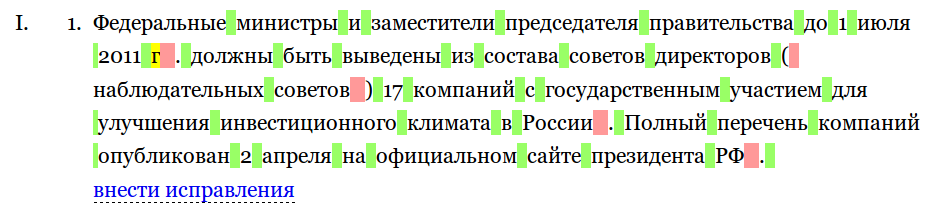
\includegraphics[width=1\linewidth]{2011_nlpseminar_2.png}}
\end{figure}
\begin{figure}
\center{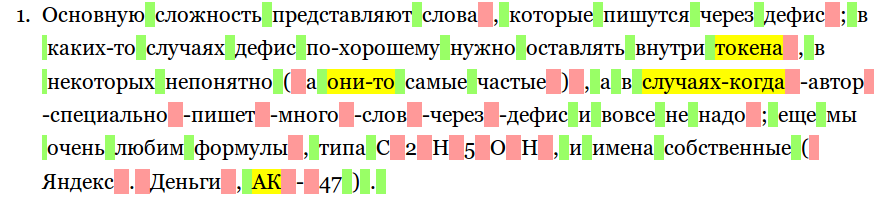
\includegraphics[width=1\linewidth]{2011_nlpseminar_3.png}}
\end{figure}
\end{frame}

%slide 08
\begin{frame}
\frametitle{Оценка качества}
\begin{itemize}
\item{Полнота / точность / F1 мера в зависимости от порога}
\begin{figure}
\center{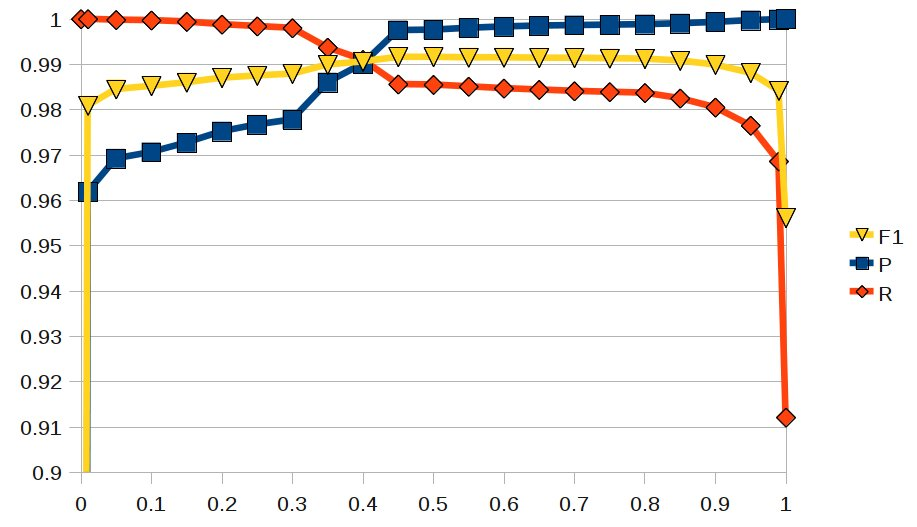
\includegraphics[width=1\linewidth]{2012_miem_3.png}}
\end{figure}
\end{itemize}
\end{frame}

%slide 09
\begin{frame}
\frametitle{Оценка качества}
\begin{itemize}
\item{При оценке не учитываются "очевидные" границы по пробелу}
\item{F1 = 99.15\% при значении порога 0.45 - 0.5}
\item{Для сравнения} \\
Правила \\
1. всегда разбивать по пробелам \\
2. всегда разбивать по границе буква / не буква \\
Дают F1 = 92\%
\end{itemize}
\end{frame}

%slide 09
\begin{frame}
\frametitle{Модуль на Perl}
\begin{itemize}
\item{Повторяет поведение токенизатора на OpenCorpora.org}
\item{Выложен на CPAN Lingua::RU::OpenCorpora::Tokenizer}
\item{Модель токенизации может обновляться}
\item{Прост в использовании:}
\begin{figure}
\center{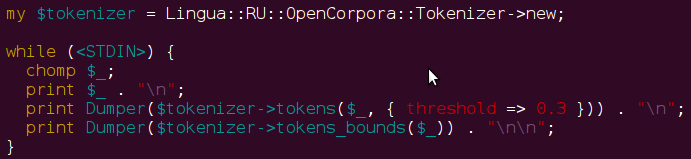
\includegraphics[width=1\linewidth]{2012_miem_1.png}}
\end{figure}
\end{itemize}
\end{frame}

%slide 10
\begin{frame}
\frametitle{Модуль на Perl}
\begin{itemize}
\item{Результат работы модуля:}
\begin{figure}
\center{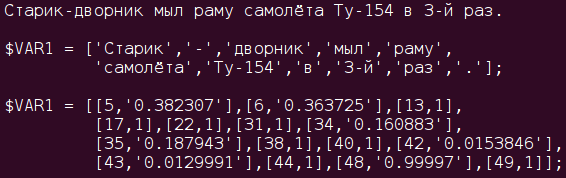
\includegraphics[width=1\linewidth]{2012_miem_2.png}}
\end{figure}
\end{itemize}
\end{frame}

%slide 10 
\begin{frame}
\frametitle{Контакты}
\begin{center}
\LARGE http://opencorpora.org\\[\bigskipamount]
\Large http://vk.com/opencorpora\\
\Large http://twitter.com/opencorpora\\
\Large http://groups.google.com/group/opencorpora/\\[\bigskipamount]
\Large\texttt{opencorpora@opencorpora.org}
\end{center}
\end{frame}

\end{document}
